\externaldocument{scala}
\chapter{Implementierung}\label{chap:Implementierung}

\section{Aufbau der GUI}
Um die benötigten Zeichen- Kontroll- und Schaltflächen zu unserem Interface hinzuzufügen, haben wir uns für die Sprache
FXML entschieden. Dabei hat unsere Applikation folgenden Aufbau:
Auf der untersten Ebene befinden sich eine \texttt{MenuBar}, welche das Menü in der oberen Leiste
einer Standardandwendung darstellt und eine \texttt{BorderPane}, die es erlaubt, das eigentliche
Fenster zur Visualisierung des Mergesort in verschiedene Bereiche zu unterteilen. Im oberen Bereich der \texttt{BorderPane}
befindet sich eine \texttt{AnchorPane}, die dazu dient, das Anordnen der Schalt- und Kontrollflächen zu erleichtern, da diese dort
relativ zu den Rändern und anderen Elementen ausgerichtet werden können.


\begin{figure}[!htb]
    \centering
      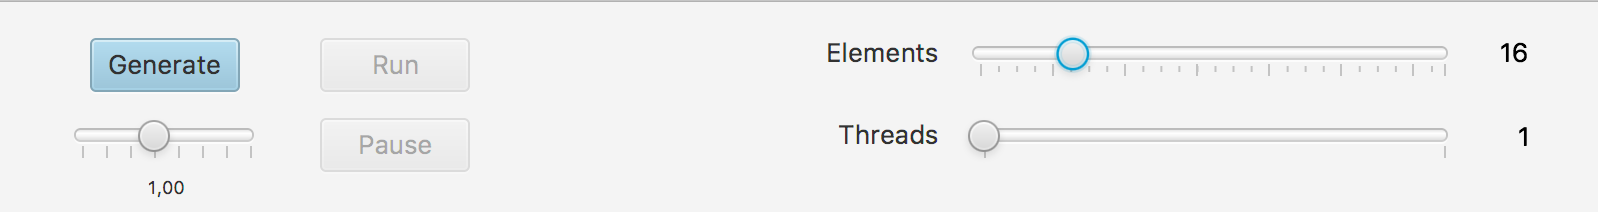
\includegraphics[width=0.75\linewidth]{bild3}
    \caption{Anchorpane mit Schaltflächen}
\end{figure}

Im Zentrum der \texttt{BorderPane} befindet sich eine \texttt{ScrollPane}, die alle weiteren Elemente beinhaltet,
die zur Darstellung der eigentlichen Zeichenfläche dienen. In diesem Teil finden ausschließlich die Animationen statt - somit sind keine Interaktionen mit der
Benutzeroberfläche möglich.

\begin{figure}[!htb]
    \centering
      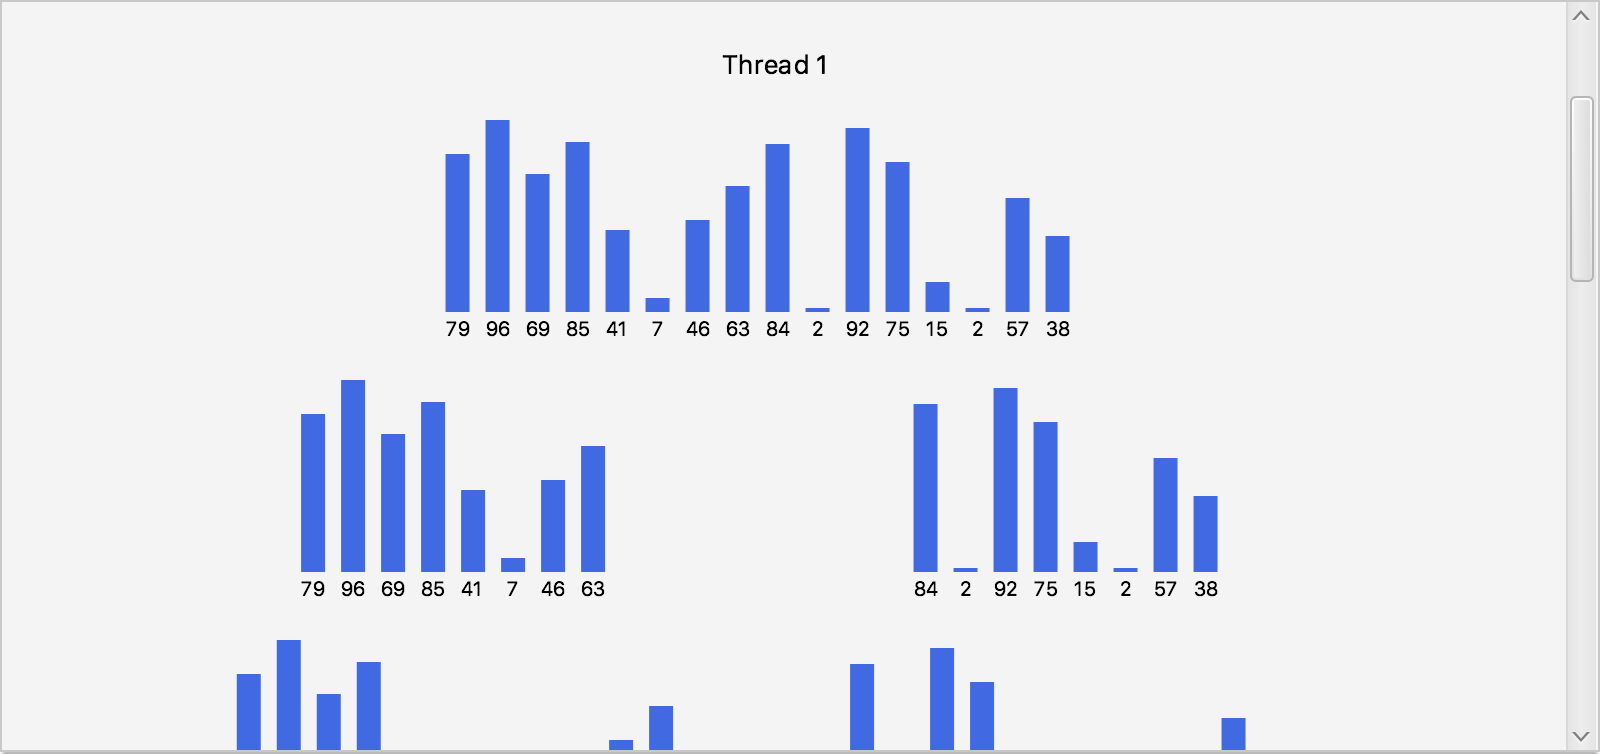
\includegraphics[width=0.75\linewidth]{bild4}
    \caption{Scrollpane mit generierten Elementen}
\end{figure}

Zuletzt befindet sich im unteren Teil der \texttt{BorderPane} eine \texttt{TextArea}, die für alle textuellen Ausgaben in der Konsole
verantwortlich ist. Hier kann der Benutzer optionalerweise das Geschehen, welches im Zentrum animiert wird,
auf leserische Art mitverfolgen.

\begin{figure}[!htb]
    \centering
      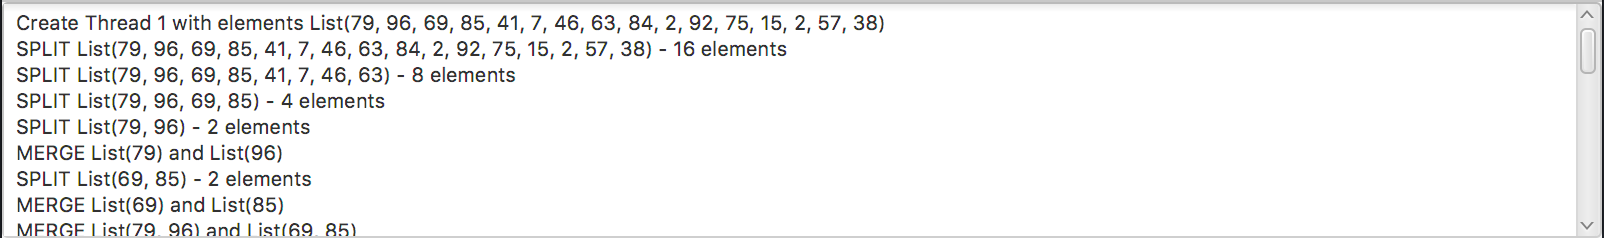
\includegraphics[width=0.75\linewidth]{bild5}
    \caption{Textarea als Konsole}
\end{figure}

\section{Das Objekt VisualMergesort}
Das Objekt VisualMergesort ist ein Singleton-Objekt der anonymen Klasse VisualMergesort, welches garantiert einzigartig ist. Das bedeutet, dass keine weiteren Objekte gleicher Art erzeugt werden können. „VisualMergesort“ erbt von JFXApp und definiert somit den Startpunkt unserer Applikation.

\begin{lstlisting}[language=Scala]
import java.io.IOException

import scalafx.application.JFXApp
import scalafx.application.JFXApp.PrimaryStage
import scalafx.scene.Scene
import scalafx.Includes._
import scalafxml.core.{FXMLView, NoDependencyResolver}
object VisualMergesort extends JFXApp {

  private val layoutFile: String = "/VisualMergesort.fxml"
  val resource = getClass.getResource(layoutFile)

  if (resource == null) {
    throw new IOException(s"Cannot load resource: $layoutFile")
  }

  val root = FXMLView(resource, NoDependencyResolver)

  stage = new PrimaryStage() {
    title = "Visual Mergesort"
    scene = new Scene(root)
  }

}
\end{lstlisting}

In diesem Objekt wird das in FXML vordefinierte Layout unserer GUI in die Stage der Applikation geladen.

\section{Die Klasse SortElement}
Die Klasse SortElement ist für die Objekte verantwortlich, die durch den Algorithmus auf der Zeichenfläche sortiert werden sollen. Die zu sortierenden Objekte sind zusammengesetzte Gruppen und bestehen aus einem Rechteck sowie einem darunter liegenden Text, welcher den Wert des Objektes angibt. Die Höhe des Rechtecks verhält sich proportional zu diesem Wert.
Der Text benötigt, um mittig unter dem Rechteck zu stehen, noch einen offset, falls der Wert einstellig ist.

Über das \texttt{require} werden Voraussetzungen für die Klasse angegeben, die zu Exceptions führen, wenn diese nicht korrekt sind.

\begin{lstlisting}[language=Scala,caption=Kopf der SortElement Klasse]
class SortElement(val number: Int, var _xPos: Double, var _yPos: Double) extends Group with Ordered[SortElement]  {
  require(number >= 1 && number <= 99 , "the number must be between 1 and 99 (inclusive)")

  var text = new Text(number.toString)
  text.style = "-fx-font-size: 10px; -fx-background: #f00"

  val offset = if (number < 10) { SortElement.smallNumberOffset } else { 0 }
  text.translateX() = xPos + offset
  text.translateY() = _yPos + number + SortElement.width

  var rectangle = new Rectangle(new javafx.scene.shape.Rectangle(_xPos, _yPos, SortElement.width, number))
  rectangle.setFill(Color.DARKBLUE)
  this.getChildren.addAll(rectangle,text)
\end{lstlisting}

Um die von Scala vordefinierten Getter und Setter der Variablen \texttt{xPos} und \texttt{yPos} zu überschreiben, werden diese in \texttt{\_xPos} und
\texttt{\_yPos} umbenannt. Danach werden zunächst die Getter definiert:

\begin{lstlisting}[language=Scala,caption=Definiert die Setter Methoden]
def xPos = _xPos
def yPos = _yPos
\end{lstlisting}

Dieser Code definiert zwei simple Methoden \texttt{xPos} und \texttt{yPos}, welche die Variablen \texttt{\_xPos} und \texttt{\_yPos} zurückgeben. Da bei Scala der letzte Ausdruck einer Methode auch gleichzeitig der Rückgabewert ist und geschweifte Klammern nicht benötigt werden, falls die Methode nur aus einem Ausdruck besteht, sind diese und das Return-Statement nicht vorhanden.

Als nächstes werden die Setter neu definiert:

\begin{lstlisting}[language=Scala,caption=Setter Methoden]
def xPos_= (x: Double) {
  _xPos = x
  text.translateX = _xPos + offset
  rectangle.x = x
}

def yPos_= (y: Double) {
  _yPos = y
 text.translateY = _yPos + number + SortElement.width
  rectangle.y = y
}
\end{lstlisting}

Der Name dieser Methoden ist \texttt{xPos\_} und \texttt{yPos\_}. Der Unterstrich dient in Scala als spezielles Zeichen und ist in diesem Fall als Platzhalter zu verstehen, der beim Aufrufen der Methoden durch ein Leerzeichen ersetzt werden kann. Somit können diese Methoden im folgenden Code sowohl mit \texttt{xPos =}  bzw. \texttt{yPos =} als auch mit \texttt{xPos\_=} bzw. \texttt{yPos\_=} aufgerufen werden. Siehe \ref{sec:getter-and-setter}

Um die Objekte beim Sortieren durch den Mergesort miteinander vergleichen zu können, werden die Methoden des Trait \texttt{Ordered} implementiert. Dieser Trait entspricht dem Interface \texttt{Comparable} in Java. Zusätzlich zu der Methode \texttt{compare} werden verschiedene Vergleichsoperatoren für das Objekt SortElement neu definiert:

\begin{lstlisting}[language=Scala,caption=Überschriebene Methoden]
override def compare(that: SortElement): Int = {
  this.number - that.number
}

override def <(that: SortElement): Boolean = {
  this.number < that.number
}

override def <=(that: SortElement): Boolean = {
  this.number <= that.number
}

override def >(that: SortElement): Boolean = {
  this.number > that.number
}

override def >=(that: SortElement): Boolean = {
  this.number > that.number
}

override def toString(): String = {
  this.number.toString
}
\end{lstlisting}

Zusätzlich zu der Klasse SortElement wird noch ein \texttt{Singleton-Object} \texttt{SortElement} angelegt, welches alle vordefinierten Werte beinhaltet, die von der Klasse SortElement benötigt werden. Die Klasse SortElement kann auf alle Felder des Objektes zugreifen und diese für Erstellung neuer Objekte benutzen.

\begin{lstlisting}[language=Scala,caption=Das Singleton--Object SortElement]
object SortElement{
  // To place small numbers (numbers < 10) centered under the rectangle, this offset is needed.
  val smallNumberOffset = 3
  // This is the rectangles width
  val width = 12
  // This is the space between two rectangles
  val offsetToNextElement = 8

  val wholeElementWidth = width + offsetToNextElement

  val maxHeight = 99
  val minHeight = 1
}
\end{lstlisting}

\section{Die Klasse MainController}

Die Klasse MainController ist, wie der Name schon hergibt, der Controller unserer Applikation. Hier werden alle Interaktionen des Benutzers mit der GUI entgegengenommen und verarbeitet. Um dies zu implementieren, werden alle im FXML-Layout vordefinierten Buttons, Slider und andere Eingabemöglichkeiten in diese Klasse importiert und deren Methoden definiert. Hierzu dient die über der Klasse stehende Annotation \texttt{@sfxml} . Die Objekte lassen sich über eine im FXML-Code festgelegte ID vom Controller ansprechen. Diese ID’s müssen für die Klasse übernommen und am Anfang festgelegt werden:

\begin{lstlisting}[language=Scala,caption=Erzeugen der Elemente und Initialisierung der Anwendung durch den Benutzer]
@sfxml
class MainController(
                      private val generateButton: Button,
                      private val runButton: Button,
                      private val amountOfElementsSlider: Slider,
                      private val amountOfThreadsSlider: Slider,
                      private val amountOfElementsLabel: Text,
                      private val amountOfThreadsLabel: Text,
                      private val playPauseMenu: MenuItem,
                      private val playPauseButton: Button,
                      private val playbackSpeed: Slider,
                      private val playbackSpeedLabel: Label,
                      private val consoleLog: TextArea,
                      private val borderPane: BorderPane,
                      private val scrollPane: ScrollPane,
                      private val pane: Pane,
                      private val actionBar: AnchorPane) {
\end{lstlisting}

Um den Visual-Mergesort betriebsbereit zu machen, hat der Benutzer die Möglichkeit, aus drei verschiedenen Möglichkeiten auszuwählen, um die zu sortierenden Elemente auf der Zeichenfläche zu platzieren. Im Menü lässt sich über die vorhandenen Schaltflächen auswählen, ob die Elemente vom System zufällig verteilt, vorsortiert oder invertiert erzeugt werden sollen. Hierzu dient ein Enum, das je nach betätigtem Button mit dem entsprechenden Wert an die Methode \texttt{generateNumbers} übergeben wird.

\begin{lstlisting}[language=Scala]
def generateRandomNumbers(): Unit = {
  generateNumbers(ElementOrder.Random)
  changeButtonActivationToRun()
}

def generateOrderedNumbers(): Unit = {
  generateNumbers(ElementOrder.Ordered)
  changeButtonActivationToRun()
}

def generateInverseNumbers(): Unit = {
  generateNumbers(ElementOrder.Inverse)
  changeButtonActivationToRun()
}
\end{lstlisting}

Nachdem die Elemente erzeugt wurden, ist die Anwendung betriebsbereit und der Run-Button wird aktiviert.

In der Methode \texttt{generateNumbers} wird eine Liste mit Zufallszahlen zwischen dem Minimalwert \texttt{defaultMinimumNumber} und dem Maximalwert \texttt{defaultMaximumNumber} generiert, die so viele Elemente enthält, wie über den Slider in der Applikation eingestellt wurde. Der Unterstrich dient in diesem Fall als Platzhalter für jedes Element in der Liste. Je nachdem, welcher Button zuvor betätigt wurde, wird die Liste  anschließend optional noch sortiert oder invertiert.

\begin{lstlisting}[language=Scala,caption=Erstellung der Zahlen-Elemente]
def generateNumbers(elementOrder: EnumVal): Unit = {

  // Get the selected amount of elements
  val amountOfElements: Integer = amountOfElementsLabel.text().toInt

  val randomNumberList = List.tabulate(amountOfElements)(_ => ThreadLocalRandom.current.nextInt(defaultMinimumNumber, defaultMaximumNumber + 1))
  val elements = elementOrder match {
    case ElementOrder.Random => randomNumberList
    case ElementOrder.Ordered => randomNumberList.sorted
    case ElementOrder.Inverse => randomNumberList.sorted.reverse
    case _ => throw new IllegalArgumentException(s"$elementOrder is not supported")
  }

  placeElementsOnPane(elements)
}
\end{lstlisting}

Zum Schluss wird die fertige Liste and die Methode \texttt{placeElementsOnPane} übergeben.

Die Methode \texttt{placeElementsOnPane} erzeugt für jeden Wert in der übergebenen Liste ein \texttt{SortElement} und fasst alle generierten Objekte in einer Gruppe zusammen. Ist die Applikation bei Aufruf der Methode am Laufen, wird sie gestoppt.

\begin{lstlisting}[language=Scala]
  def placeElementsOnPane(elements: List[Int]): Unit = {

    cleanEverythingUp
    // Stop the running transition, and then place the new elements on the pane
    if (transition != null) transition.stop()
    // Setting up the canvas
    val elementGroup = new Group()
    elementGroup.id() = "level-1"
    // Place the elements on the pane
    for ((value, position) <- elements.zipWithIndex) {
      val xPos: Double = (position * SortElement.wholeElementWidth).toDouble
      val yPos: Double = (SortElement.maxHeight - value).toDouble
      val sortElement = new SortElement(value, xPos, yPos)
      sortElement.id() = s"sortElement-$position"
      elementGroup.children.add(sortElement)
    }

    elementGroup.translateX <== scrollPane.getScene.getWindow.width/2 - elementGroup.getBoundsInParent.getWidth/2
\end{lstlisting}

Anschließend wird die Zeichenfläche von allen darin befindlichen Objekten gesäubert und die neu generierte Gruppe wird hinzugefügt:\\
Basierend auf der Anzahl der neu erzeugten Elemente, wird die Größe der Zeichenfläche angepasst. Dazu wird vorerst die maximale Tiefe der Gruppen definiert. Bei jedem Split und bei jedem Merge, wandern die gesplitteten oder zusammengesetzten Gruppen eine Ebene nach unten. Da sich eine Gruppe bei jedem Split so lange in zwei Teile teilt, bis sich nur noch ein einziges Element in der Gruppe befindet und genauso viele Merges wie Splits durchgeführt werden, lautet die Formel für die Anzahl an Splits und Merges:
$$log_2 n \times 2$$

Allerdings befindet sich von Anfang an schon die vom System generierte Gruppe auf der Zeichenfläche. Diese muss noch hinzugerechnet werden. Somit ergibt sich für die maximale Tiefe

$$log_2 n \times 2 + 1$$

\begin{lstlisting}[language=Scala]
pane.children.clear()
pane.children.add(elementGroup)
pane.setPrefWidth(elementGroup.getBoundsInParent.getWidth)
scrollPane.vvalue = 0.0

val depth = Math.ceil(Math.log(elementGroup.children.size) / Math.log(2)) * 2 + 1
pane.setPrefHeight(depth * 130)
\end{lstlisting}

Wurde die zu sortierende Menge auf der Zeichenfläche platziert, kann der Benutzer auf „Run“ klicken, um den Algorithmus zu starten. Dadurch wird die Methode \texttt{runSorting} ausgeführt.

\begin{lstlisting}[language=Scala,caption=runSorting startet die Sortierung mit anschließender Animationen]
def runSorting():Unit = {
  runButton.disable = true
  isPlaying() = true
  playPauseMenu.disable = false
  playPauseButton.disable = false
  val elementGroup: javafx.scene.Group = pane.children.get(0).asInstanceOf[javafx.scene.Group]

  val sorter = new SortElementsController(pane, consoleLog)
  sorter.maxDepth =  Math.ceil(Math.log(elementGroup.children.size) / Math.log(2)) * 2 + 1
  sorter.sort(elementGroup, 0)
  transition = sorter.getSequence
  transition.rate <== MathBindings.pow(2.0, playbackSpeed.value)

  transition.play()
  transition.onFinished = {
    event: ActionEvent =>
      cleanEverythingUp
  }
}
\end{lstlisting}

Durch die Methode \texttt{runSorting} wird der Run-Button deaktiviert und der Algorithmus zum Sortieren der Elemente durchgeführt, welcher die vorher generierte Gruppe als Eingangsmenge übernimmt. Anschließend wird die Animation, die den Algorithmus visualisiert, gestartet.

Die Implementierung der Logik für den Algorithmus befindet sich in der Klasse \texttt{Sort""Elements""Controller}.

Wie schon erwähnt, wird bei unserer Implementierung des Mergesort-Algorithmus nicht mit einer einzigen Gruppe gearbeitet, sondern mit vielen Listen, die nicht überschrieben werden. Das dient dazu, die schon gesplitteten und gemergten Elemente auf der Zeichenfläche unangetastet zu lassen. Um dies zu realisieren, müssen Duplikate der Eingangslisten erstellt werden, mit denen weitergearbeitet werden kann, ohne die schon gezeichneten Objekte zu beeinflussen. Man braucht also eine zweite Liste, welche Objekte mit äquivalenten Werten enthält. Für diese Aufgabe existiert die Methode \texttt{createGroup}, welche in unserer \texttt{sort} - Methode aufgerufen wird.

\begin{lstlisting}[language=Scala,caption=Erstellung der Gruppe]
def createGroup(parentGroup: Group, splitList: (List[SortElement], List[SortElement]), part: EnumVal, depth: Int): Group = {

  val duplicateList = (part match {
    case Part.Left => splitList._1
    case Part.Right => splitList._2
    case _ => throw new IllegalArgumentException(s"$part is not a valid argument")
  }).map(_.duplicate())

  val group = new Group() {
      opacity = 0.0
      children.addAll(duplicateList.asJava)
      translateY = parentGroup.translateY() + (if (depth > 0) moveDownByPixel else 0)
      id = s"level-${depth + 1}"
    }
    part match {
      case Part.Left =>
        group.translateX <== parentGroup.translateX - group.getBoundsInParent.getWidth / 2 + SortElement.width / 2
      case Part.Right =>
        group.translateX <== parentGroup.translateX + parentGroup.getBoundsInParent.getWidth / 2 - group.getBoundsInParent.getWidth/2 - SortElement.width/2

    }
  group
}
\end{lstlisting}

Die Methode createGroup erzeugt gleich zu Beginn ein Duplikat der eingegangenen splitList und zwar, abhängig vom mitgegebenem Enum, entweder von der linken oder der rechten Hälfte und speichert dieses in der Value \texttt{duplicateList}. Die \texttt{map}--Methode, die hier verwendet wird, erzeugt für jedes SortElement-Objekt in einer SplitList ein Objekt mit gleichen Werten und gibt dieses an die neue Liste weiter. Der Unterstrich steht in diesem Fall also für jedes Element. Nachdem alle Elemente der „duplicateList“ zu einer Gruppe hinzugefügt wurden, wird diese Gruppe, relativ zu der Gruppe, aus der sie entstanden ist, ausgerichtet. Durch das verwendete Binding \texttt{<==} wird die Positionierung stets angepasst, falls sich die Position der Elterngruppe ändern sollte.

\section{Implementierung des Autoscrolls}
Um dem Benutzer den Fokus auf den Algorithmus zu erleichtern, haben wir es für sinnvoll erachtet, einen automatischen Scrollmechanismus zu implementieren, welcher stets das Geschehen zum Mittelpunkt der Szene macht. Hierbei machen wir uns noch einmal die zuvor für die Größe der Zeichenfläche genutzte Tiefe der Gruppenstruktur zu Nutze.

\begin{lstlisting}[language=Scala,caption=Das Autoscrolling auf der Pane]
def scroll(group: Group, depth: Int) = {
  val factor = 1.0/(maxDepth)
  val timeline = new Timeline {
    autoReverse = false
    keyFrames = Seq(
      at (0.5.s) {
        group.getScene.lookup("#scrollPaneID").asInstanceOf[ScrollPane].vvalue -> (factor * (if(depth == 0){depth} else {depth + 1}))
      }
    )
  }

  sequence.children.add(timeline)
}
\end{lstlisting}

\section{Implementierung der Animationen}

Die Methode \texttt{relocateElementGroup} erzeugt eine Animation, welche die übergebene Gruppe in 0.2 Sekunden sichtbar macht und sie binnen einer Sekunde von der Elterngruppe um einen festgelegten Wert nach unten bewegt. Hierbei ist zu beachten, dass die \texttt{threadNumber} mit an die Methode übergeben wird, da bei mehreren Threads jeder seine eigene Animationssequenz besitzt, die später parallel zu den Animationssequenzen der anderen Threads abgespielt wird.

\begin{lstlisting}[language=Scala,caption=Umpositionierung der Elemente]
def relocateElementGroup(group: Group, depth: Int, threadNumber: Int): Timeline = {
  val timeline = new Timeline {
    autoReverse = false
    keyFrames = Seq(
      at(0.2.s) {
        group.opacity -> 1.0
      },
      at(1.s) {
        group.translateY -> (group.translateY() + SortElementsController.moveDownByPixel)
      }
    )
  }
  addToSequence(threadNumber, timeline)

  timeline
}
\end{lstlisting}

Um den Threads ihre Animationen zuzuteilen, wird die Methode \texttt{addToSequence} benutzt. Hier werden zwei verschiedene Transitionen für die beiden möglichen Threads gepflegt. Zusätzlich gibt es noch eine weitere Transition, die den final merge beim Sortieren mit zwei Threads übernimmt.

\begin{lstlisting}[language=Scala,caption=Einteilung der Animationen in die entsprechende SequentialTransition]
  def addToSequence(threadNumber: Int, timeline: Timeline): Boolean = {

    if (threadNumber == 0) seq1.children.add(timeline)
    else if (threadNumber == 1) seq2.children.add(timeline)
    else {println("Adds transition to last group"); groupSeq.children.add(timeline)}
  }
  \end{lstlisting}
